\subsection{Credibility and data quality}
It is essential that the credibility of the data set be impeccable. The source of the data must be reliable. In the description of the data, a section must be included where the origin of the data set is explained.

The quality of the data set can be measured according to the following characteristics of the values of the fields: \\
 
\textbf{Precision}. Units of measurement in the correct scale. For example, if we are measuring people's height, it would be meaningless to provide these measurements in meters, since the possible values will be 0, 1 and 2. \\

\textbf{Consistency}. Logical values for each type of field. An example would be a date field, all should
follow the same format. \\

\textbf{Interpretability}. Readable. The data must be clear, both in values and in units. For example, we can not
suppose the unit or scale of the data or, if the data set is dichotomous, "true" or "false", and the values represented are
"A" or "B", we can not assume true = A and false = B without this information being described. \\

\textbf{Complitud}. The data must be consistent in each of the samples. The samples can be differentiated
  from each other, as we see in the Figure below, can share some fields and not others. It would be
better to have a high degree of compliance for the data that interests us in our design.


\begin{figure}[ht]
\centering
\framebox{
\vbox{\begin{tabbing} 
Document \\
\hspace*{5mm} \= Sample 1 \\
\hspace*{10mm}\textit{Field A:} \hspace*{5mm} \= value A \\
\hspace*{10mm}\textit{Field B:} \hspace*{5mm} \= value B \\
\hspace*{5mm} \= Sample 2 \\
\hspace*{10mm}\textit{Field A:} \hspace*{5mm} \= value A \\
\hspace*{10mm}\textit{Field C:} \hspace*{5mm} \= value C \\
\hspace*{10mm}\textit{Field D:} \hspace*{5mm} \= value D \\
\hspace*{5mm} \= ... 
\hspace*{5mm} \= Sample n \\
\hspace*{10mm} \= ... 
\end{tabbing}}%
}
\caption{Example source source document}
\end{figure}

\subsubsection{How to solve it} 
The first step is to compare the information with the source of origin. With the data set and the definition
of each of the fields, the scale and interpretability of the fields and values must be checked.
Then we can perform different analysis of the data to check its consistency and compliance.
It is possible to use different graphs and see if there are extreme or strange values.
Database analysis tools can tell us the completeness of the fields, that is, what percentage of the
samples contain each field.

\subsubsection{How we solve it. Aire Guru} 
The source of data is verified by both the CEMI (Malaga information center) and UrbanClouds, the private company
that collects and sends the data to the city of Malaga.
With the description of the data in the open data portal of Malaga and the information received by UrbanClouds,
we obtain all the necessary information to interpret the data set. \\

For each field, a graphical study has been carried out with the Tableau tool and has verified that the values of the
fields meet the scale and range of expected values, that is, they are precise and consistent.
Using the analysis tools of MongoDBCompas and NoSQLBooster we verify the completeness of the fields needed for our model.
\begin{figure}[ht]
    \centering
    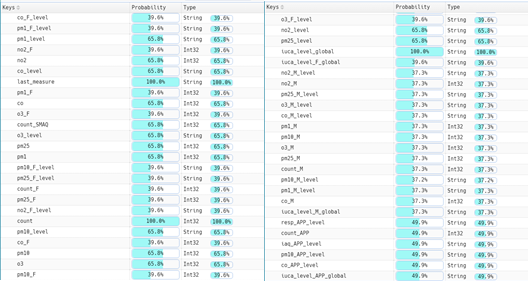
\includegraphics[width=12cm]{noSQLBoosterAnalysis}
    \caption{Completeness analysis}
\end{figure}

\elsparagraph{Evaluation}  
\begin{itemize}
    \done The necessary measures have been taken to verify and understand each of the fields in the data set.
    \done The values of each of the fields have been analyzed by checking scales and ranges.
    \done The completeness of the data has been analyzed.
    
\end{itemize}
 \newpage